% LaTeX Beamer From Scratch
%%
% Andre Pereira andrespp at gmail dot com
% 13/10/2009
%
% This document is based on the Beamer User Guide, available at:
% http://www.ctan.org/tex-archive/macros/latex/contrib/beamer/doc/beameruserguide.pdf

%Todo/Learn:
% * Capa (Orientador)
%	* Sumario
% * Referencias

\documentclass{beamer}

%%%Style setup
%\usetheme{Madrid} 	% Very clean
%\usetheme{Antibes}	% 3 top bars: section, subsection, subsubsection
\usetheme{Frankfurt}	% 2 top bars: section, slide counter %%esse
%\usetheme{Ilmenau}
%\usetheme{Berlin}	% 2 top bars: section, slide counter
%\usetheme{Warsaw}	% large top bar
%\usetheme{Bergen} 	% left side bar (uhhg)
%\usetheme{Rochester} 	% clean with large top bar
%\usetheme{Darmstadt}
%\usetheme{Boadilla}	% super clean
%\usetheme{Copenhagen}
%\usetheme{Dresden}	% 2 top bars
%\usetheme{Malmoe}
%\usetheme{Goettingen}	% clear right bar
%\usetheme{Hannover}	% clear left bar
%\usetheme{Ilmenau}
%\usetheme{JuanLesPins}	% 3 top bars (slim)
%\usetheme{Luebeck}
%\usetheme{Marburg}	% bold right bar
%\usetheme{PaloAlto}	% left / top bar
%\usetheme{Singapore}	% clear top bar
%\usetheme{Szeged}
%\usetheme{default}	% totaly white background
%\usetheme{Montpellier}

%\usecolortheme{seahorse}	%diminui o contraste
%\usecolortheme{rose}			%diminui o contraste
%\usefonttheme[onlylarge]{structuresmallcapsserif}

% Hide slide bullets on header
\setbeamertemplate{headline}
 {%
  \begin{beamercolorbox}{section in head/foot}
  \insertsectionnavigationhorizontal{\textwidth}{}{}
  \end{beamercolorbox}%
}


%%%Package Setup
\usepackage[brazil]{babel}
\usepackage[utf8]{inputenc} 	%uso de acentos - linux
%\usepackage[latin1]{inputenc} %uso de acentos - windows
\usepackage{listings}
\usepackage{subfig}

%%%Document Setup
\mode<presentation>
\title{\textit{Green-Markov models - new optimization strategies: a case study
for user allocation in co-channel macro/femto networks}}
%\subtitle{Trabalho da Disciplina PPGEE0248 - Tópicos Especiais em Computação
%Aplicada}
%\author{André Augusto da Silva Pereira\\ andresp@las.ic.unicamp.br}
\author{André Pereira \\
	Daniel Victor \\
        Junior Albuquerque \\
        Sandio Maciel \\
        Thiago Ferreira \\
}
%			\textbf{Professor:} Prof. Dr. Paulo Lício de Geus}

\date{Outubro/2018}
\institute{Universidade Federal do Pará \\
Programa de Pós-Graduação em Engenharia Elétrica}

%%%Document itself
\begin{document}
%	\def\newblock{\hskip .11em plus .33em minus .07em} %bibliography fix
  \setbeamertemplate{footline}[frame number]
  \pgfdeclareimage[height=0.95cm] {logo}{./Figures/ufpa}
	\logo{\pgfuseimage{logo}}

\begin{frame}
  \titlepage
\end{frame}

\section{Introdução}

\begin{frame}{Agenda}
	\tableofcontents
\end{frame}
\frame{\tableofcontents[currentsection]}

\begin{frame}
  \begin{block}{Contexto}
    \begin{itemize}
      \item Crescimento explosivo de comunicações sem fio
      \begin{itemize}
        \item Redes ubíquas
        \item Em Dez/2011 Brasil possuía $~242.2$ milhões de telefones
        celulares ($~123,87/100$ habitantes)
      \end{itemize}
      \item Neste contexto, as \textit{\alert{Femtocells}} podem ser utilizadas
      para melhorar os serviços de voz %em uma área de cobertura limitada
    \end{itemize}
  \end{block}
  \begin{figure}[h]
  	\begin{center}
      \includegraphics [scale=0.18]{./Figures/FemtocellTopology}
      \caption {Cenário Típico de utilização de \textit{Famtomcells}
      \cite{green-markov}.}
  		\label{fig:FemtocellTopology}
  	\end{center}
  \end{figure}
\end{frame}

\begin{frame}
  \begin{block}{Desafios}
    \begin{enumerate}
      \pause
      \item \alert{Escalonamento em cenários Macro-femtocell}
        \begin{itemize}
          %\item Múltiplas \textit{femtocell} vs \textit{macro-cell},
          %tipicamente co-canal
          \item Tipicamente \textit{femtocells} e \textit{macrocells} utilizam
          o mesmo espectro (co-canal)
          \item Balanceamento de carga (concentração inadequada de clientes em
          algumas \textit{femtocells}
        \end{itemize}
      \pause
      \item \alert{Aspectos de qualidade}
        \begin{itemize}
          \item Consumo de bateria de clientes
          \item Requisitos de QoS devem direcionar a escolha da conexão
        \end{itemize}
      \pause
      \item \alert{Consumo eficiente de energia}
        \begin{itemize}
          \item Efeito estufa
          \item Estima-se que $~57\%$ do consumo de energia em sistemas de TIC
          são gerados por clientes e dispositivos de redes móveis
        \end{itemize}
    \end{enumerate}
  \end{block}
\end{frame}

\begin{frame}
  \begin{block}{Proposta}
    \begin{itemize}
      \item \alert{Alocação ótima} de usuários em redes \textit{macro-femto}
      co-canais, permitindo \alert{auto-configuração}, com o objetivo de
      \alert{maximizar a qualidade de serviço} para as aplicações, e
      proporcionar um \alert{consumo eficiente} de energia.
    \end{itemize}
  \end{block}
\end{frame}

%\begin{frame}
%  \begin{block}{}
%    \begin{itemize}
%      \item
%    \end{itemize}
%  \end{block}
%\end{frame}

%\begin{frame}
%  \begin{block}{}
%  \end{block}
%\end{frame}

%\begin{frame}
%  \begin{figure}[h]
%  	\begin{center}
%      \includegraphics [scale=0.3]{./Figures/Device-Estimates}
%     % \caption {Estimativa de dispositivos conectados à Internet.}
%  		%\label{fig:arq-imuno}
%  	\end{center}
%  \end{figure}
%\end{frame}

%\begin{frame}{Redes de Acesso}
%	\begin{figure}[!htb]
%		\centering
%		\subfloat[DSL]{
%			\includegraphics[height=3.5cm]{./Figures/DSLaccess}
%			\label{figdroopy}}
%		\quad %espaco separador
%		\subfloat[Cable]{
%			\includegraphics[height=3.5cm]{./Figures/CableAccess}
%			\label{figsnoop}}
%		%\caption{Subfiguras}
%		%\label{fig01}
%	\end{figure}
%\end{frame}

%\begin{frame}[fragile]
%\scriptsize
%\begin{verbatim}
%\end{verbatim}
%\end{frame}


\section{Femtocell}
\frame{\tableofcontents[currentsection]}
\begin{frame}
  \begin{block}{Características}
    \begin{itemize}
      \item Pontos de acesso de baixos alcance, custo, consumo de energia
      \item \textit{aka \alert{home base-stations}}
      \item Ajudam a melhorar a cobertura em pequenas áreas%, conectando
      %localmente redes celulares e roteando o tráfego através da Internet
      \item \textit{Bridge} entre o usuário e a rede da operadora usando a
      Internet
    \end{itemize}
  \end{block}
	\begin{figure}[!htb]
		\centering
		\subfloat[Femtocell]{
			\includegraphics[height=3.5cm]{./Figures/Femtocell}
			\label{figdroopy}}
		\quad %espaco separador
		\subfloat[Macrocells]{
			\includegraphics[height=3.5cm]{./Figures/Macrocell}
			\label{figsnoop}
			\includegraphics[height=2.5cm]{./Figures/Macrocell2}
			\label{figsnoop}}
		%\caption{Subfiguras}
		%\label{fig01}
	\end{figure}
\end{frame}

\begin{frame}
  \begin{figure}[h]
  	\begin{center}
      \includegraphics [scale=0.35]{./Figures/FemtocellTopology}
      \caption {Cenário Típico de utilização de \textit{Famtomcells}
      \cite{green-markov}.}
  		\label{fig:FemtocellTopology}
  	\end{center}
  \end{figure}
\end{frame}

\begin{frame}
  \begin{block}{Vantagens}
    \begin{itemize}
      \item Melhor cobertura de sinal (ambientes de difícil acesso, ambientes
      \textit{indoor}, etc...)
      \item Tipicamente instalados por não-especialistas
      \item Auto-organização dos parâmetros operacionais
      \item Cliente se associa automaticamente a \textit{femtocell} de melhor
      potência de sinal
    \end{itemize}
  \end{block}

  \begin{block}{Desvantagens da associação por potência de sinal}
    \begin{itemize}
      \item Possibilidade de sobrecarga de células
      \item Mau balanceamento de clientes entre células
      \item A escolha pode não atender critérios de QoS demandadas pela
      aplicação
    \end{itemize}
  \end{block}
\end{frame}

%\begin{frame}
%  \begin{block}{}
%    \begin{itemize}
%      \item
%    \end{itemize}
%  \end{block}
%\end{frame}

%\begin{frame}
%  \begin{block}{}
%  \end{block}
%\end{frame}

%\begin{frame}
%  \begin{figure}[h]
%  	\begin{center}
%      \includegraphics [scale=0.3]{./Figures/Device-Estimates}
%     % \caption {Estimativa de dispositivos conectados à Internet.}
%  		%\label{fig:arq-imuno}
%  	\end{center}
%  \end{figure}
%\end{frame}

%\begin{frame}{Redes de Acesso}
%	\begin{figure}[!htb]
%		\centering
%		\subfloat[DSL]{
%			\includegraphics[height=3.5cm]{./Figures/DSLaccess}
%			\label{figdroopy}}
%		\quad %espaco separador
%		\subfloat[Cable]{
%			\includegraphics[height=3.5cm]{./Figures/CableAccess}
%			\label{figsnoop}}
%		%\caption{Subfiguras}
%		%\label{fig01}
%	\end{figure}
%\end{frame}

%\begin{frame}[fragile]
%\scriptsize
%\begin{verbatim}
%\end{verbatim}
%\end{frame}


\section{Conceitos de Modelos Markovianos}
\frame{\tableofcontents[currentsection]}
\begin{frame}
  \begin{block}{Definições}
    \begin{itemize}
      \pause
      \item \alert{\textit{Markov Decision Process} - MDP}
      \begin{itemize}
        \item Ferramenta matemática utilizada para analizar sistemas
        \alert{reativos} complexos e definir \alert{políticas} que minimizem o
        \alert{custo} operacional
      \end{itemize}
      \pause
      \item \alert{\textit{Continuous Time MDP} - CTMDP}
      \begin{itemize}
        \item MPD onde os eventos ocorrem a tempo contínuo (ou seja, a qualquer
        tempo)
      \end{itemize}
      \pause
      \item \alert{Infinite Horizon Problem}
      \begin{itemize}
        \item Processos que persistem por um longo período de tempo
      \end{itemize}
    \end{itemize}
  \end{block}
  \pause
  Este trabalho implementa um modelo do tipo \textit{\textbf{Infinite Horizon
  CTMDP}}
\end{frame}

\begin{frame}
  \begin{block}{Modelagem de um CTMDP}
    \begin{itemize}
      \pause
      \item \alert{\textit{The state space:}} $S$
      \begin{itemize}
        \item Conjunto de todos os estados possíveis
      \end{itemize}
      \pause
      \item \alert{\textit{Sets of actions:}} $\{ A(s) | s \in S\}$
      \begin{itemize}
        \item Para cada estado, um conjunto de todas as ações possíveis
      \end{itemize}
      \pause
      \item \alert{\textit{A set of costs:}} $\{c(s,a) | s \in S, a \in A(s) \}$
      \begin{itemize}
        \item Custo associado a ação $a$ quando o sistema está no
        estado $s$
      \end{itemize}
      \pause
      \item \alert{\textit{A set of transitions probabilities:}}
      $ \{ p_{sz}(a) | s,z \in S, a \in A(s) \}$
      \begin{itemize}
        \item Probabilidade de, no próximo instante de decisão, o sistema estar
        no estado $z$ dado ter tomado a ação $a$ no instante em que
        encontrava-se no estado $s$
      \end{itemize}
      \pause
      \item \alert{\textit{Expected time until next decision:}}
      $ \{ \pi (s,a) | s \in S, a \in A(s) \}$
      \begin{itemize}
        \item Considerando que a ação $a$ foi escolhida no estado $s$
      \end{itemize}
    \end{itemize}
  \end{block}
  \pause
  A partir destas definições, pode-se calcular um política $R*$ que minimiza a
  média da função custo
\end{frame}

\begin{frame}
  \begin{block}{Transição de estados é uma função dependente do tempo}
    \begin{itemize}
      \item Um evento ocorre em um instante $t_n$
      \item Depois do evento, o estado do sistema muda e, simultaneamente, uma
      decisão é tomada
      \item Entre os instantes $t_n$ e $t_{n+1}$, o comportamento do sistema
      irá depender de ambos estados e ação em $t_n$
    \end{itemize}
  \end{block}
\end{frame}

\begin{frame}
  \begin{figure}[h]
  	\begin{center}
      \includegraphics [scale=0.3]{./Figures/StateTransitions}
      \caption {Representação de transição de estados no tempo
      \cite{green-markov}.}
  		\label{fig:arq-imuno}
  	\end{center}
  \end{figure}
\end{frame}

%\begin{frame}
%  \begin{block}{}
%    \begin{itemize}
%      \item
%    \end{itemize}
%  \end{block}
%\end{frame}

%\begin{frame}
%  \begin{block}{}
%  \end{block}
%\end{frame}

%\begin{frame}
%  \begin{figure}[h]
%  	\begin{center}
%      \includegraphics [scale=0.3]{./Figures/Device-Estimates}
%     % \caption {Estimativa de dispositivos conectados à Internet.}
%  		%\label{fig:arq-imuno}
%  	\end{center}
%  \end{figure}
%\end{frame}

%\begin{frame}{Redes de Acesso}
%	\begin{figure}[!htb]
%		\centering
%		\subfloat[DSL]{
%			\includegraphics[height=3.5cm]{./Figures/DSLaccess}
%			\label{figdroopy}}
%		\quad %espaco separador
%		\subfloat[Cable]{
%			\includegraphics[height=3.5cm]{./Figures/CableAccess}
%			\label{figsnoop}}
%		%\caption{Subfiguras}
%		%\label{fig01}
%	\end{figure}
%\end{frame}

%\begin{frame}[fragile]
%\scriptsize
%\begin{verbatim}
%\end{verbatim}
%\end{frame}


\section{Modelo Analítico}
\frame{\tableofcontents[currentsection]}
\begin{frame}
  \begin{block}{A. Arquitetura de Rede e Previsões de Trafego}
    \begin{itemize}
      \item A chegada de novas chamadas podem ser respondidas por ambas as redes.
      \item Parâmetros usados para decidir que rede deve ser escolhida:
      \begin{itemize}
        \item Consumo de energia
        \item Vazão
        \item Probabilidade de perda de pacote
      \end{itemize}
      \item Os serviços ofertados pela rede chegam no sistema de acordo com dois processos de Poisson
      \begin{itemize}
        \item Voz ($ \lambda v _{n} $)
        \item Dados ($ \lambda d _{n} $)
      \end{itemize}
      \item Os pacotes de chamadas de voz e dados seguem uma distribuição exponencial:$ 1 / \mu v _{n} $ and $ 1 / \mu d _{n} $,respectivamente
    \end{itemize}
  \end{block}
\end{frame}

\begin{frame}
  \begin{block}{B. Formulação do Problema}
    Objetivos do modelo markoviano proposto:
    \begin{itemize}
      \item Definir a qual rede o usuário móvel deve se conectar.
      \item Minimizar os custos dos parâmetros de:
      \item \alert{Energia}
      \item \alert{Perdas de transmissão}
      \item \alert{Baixa taxa de transferência}
    \end{itemize}  
  \end{block}  
\end{frame}

\begin{frame}
  \begin{block}{Possíveis eventos:}
    \begin{itemize}
      \scriptsize
      \item \alert{$\lambda v _{m}$} e \alert{$\lambda v _{f}$} - Taxa de chegada de voz na macrocell e femtocell
      \item \alert{$\lambda d _{m}$} e \alert{$\lambda d _{f}$} - Taxa de chegada de dados na macrocell e femtocell
      \item \alert{$\lambda v _{u}$} e \alert{$\lambda d _{u}$} - Taxa de chegadas de usuários para voz e dados
      \item \alert{$\mu v _{m}$}, \alert{$\mu v _{f}$} e \alert{$\mu v _{u}$} - Taxa de serviço para voz na macrocell, femtocell e alocação dos usuários
      \item \alert{$\mu d _{m}$}, \alert{$\mu d _{f}$} e \alert{$\mu d _{u}$} - Taxa de serviço para dados na macrocell, femtocell e alocação dos usuários
    \end{itemize}
  \end{block}
  
  \begin{block}{Parâmetros do sistema:}
    \begin{itemize}
      \scriptsize
      \item \alert{$v _{m}$} e \alert{$v _{f}$} - número de conexões de voz na macrocell e femtocell
      \item \alert{$d _{m}$} e \alert{$d _{f}$} - número de conexões de dados na macrocell e femtocell
      \item \alert{$c$} - estado de conexão do usuário: macrocell($c _{m}$), femtocell($c _{f}$) ou disconectado($disc$)
      \item \alert{$k$} - tipo de aplicação: $voz$, $dados$ ou $disc$
      \item \alert{$ev$} - último evento aguardando a decisão
    \end{itemize}
  \end{block}
\end{frame}

\begin{frame}
  \footnotesize Usando esses parâmetros, cada estado \alert{s $\epsilon$ S} é definido como uma 7-tupla:
  \begin{figure}
    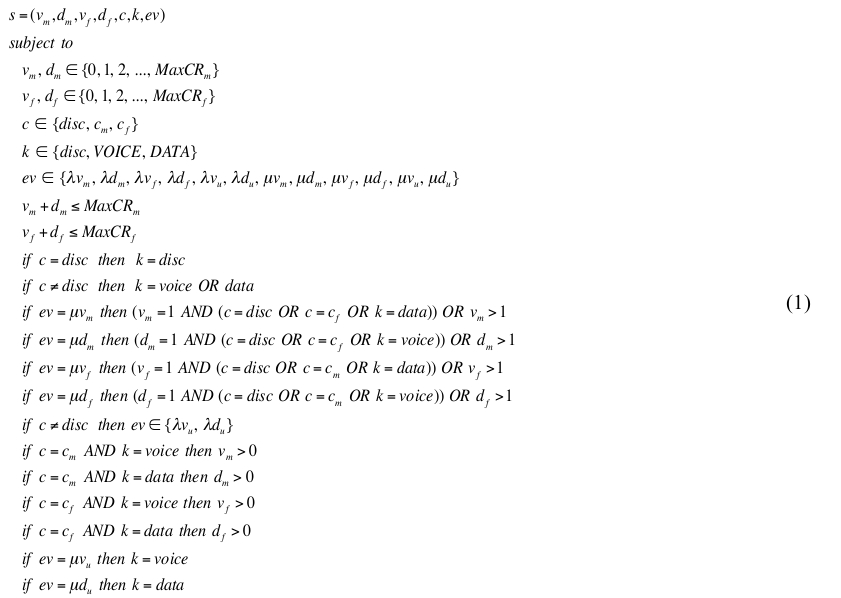
\includegraphics [scale=0.30]{./Figures/f1}
  \end{figure}
  \footnotesize Onde $MaxCR _{m}$ e $MaxCR _{f}$ são os números máximos de macrocell e femtocell, respectivamente  
\end{frame}

\begin{frame}
  \footnotesize O conjunto de possíveis ações \alert{$A(s)$} para cada estado \alert{s $\epsilon$ S} é definido como:
  \begin{figure}
    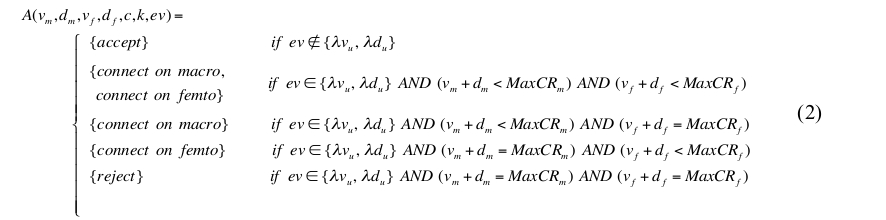
\includegraphics [scale=0.37]{./Figures/f2}
  \end{figure}  
\end{frame}

\begin{frame}
  \begin{itemize}
    \item Estados(\alert{$s _{t}$}) que podem ser alcançados a partir de \alert{$s _{f}$}
  \end{itemize}    
  \begin{figure}
    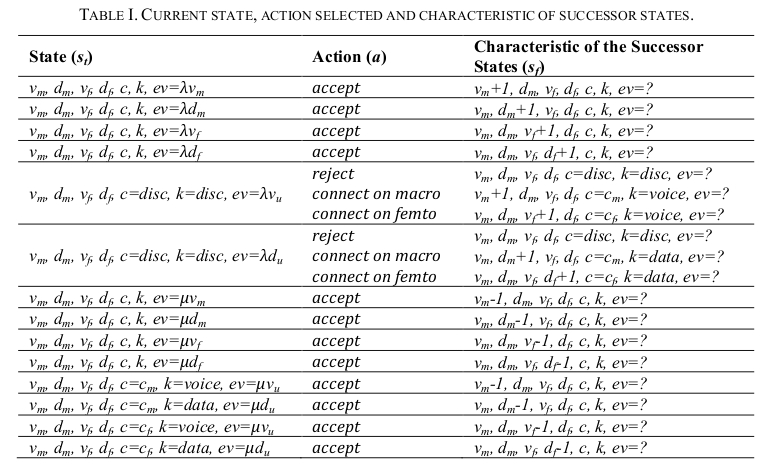
\includegraphics [scale=0.37]{./Figures/f3}
  \end{figure}  
\end{frame}

\begin{frame}
  \begin{itemize}
    \item Identificação dos possíveis estados que podem ser alcançados a partir de \alert{$s _{f}$}
  \end{itemize}    
  \begin{figure}
    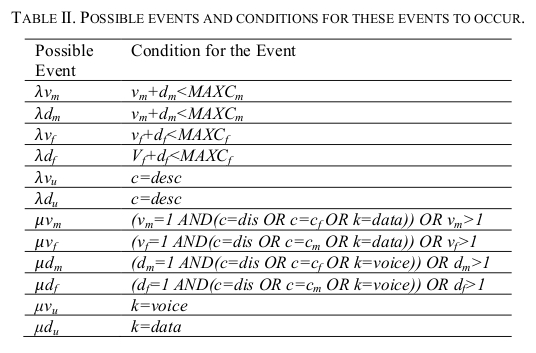
\includegraphics [scale=0.37]{./Figures/f4}
  \end{figure}  
\end{frame}

\begin{frame}{\small Como todos os eventos são representados por um processo de Poisson}
    \begin{itemize} 
      \item \footnotesize Cálculo da taxa de saída total \alert{$s _{f}$}, quando a ação \alert{$a$} é selecionada:
    \end{itemize} 
     
    \begin{figure} 
      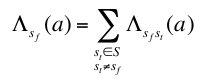
\includegraphics[scale=0.37]{./Figures/form1} 
      \scriptsize , onde $\Lambda _{sf st}$ é a taxa de transição do estado $s_{f}$ para o estado $s_{t}$.
    \end{figure}  
    
    \begin{itemize}
      \item \footnotesize Cálculo da probabilidade de transição:
    \end{itemize}
    
    \begin{figure} 
      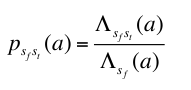
\includegraphics[scale=0.37]{./Figures/form2} 
    \end{figure}
    
    \begin{itemize}
      \item \footnotesize Cálculo do tempo esperado até a próxima decisão:
    \end{itemize}
    
    \begin{figure} 
      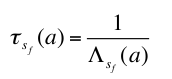
\includegraphics[scale=0.37]{./Figures/form3} 
    \end{figure}
\end{frame}

\begin{frame}
  \footnotesize Os custos utilizados pelo sistema quando este está no estado de \alert{$s_{f}$} e uma acção \alert{$a$} é escolhido, pode ser calculado por:
  \begin{figure}
    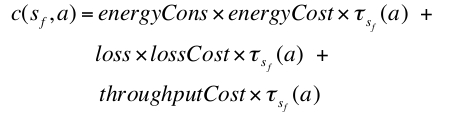
\includegraphics[scale=0.37]{./Figures/form4}
  \end{figure}
  \scriptsize Onde:
  \begin{itemize}
    \item \alert{$energyCons$} é o consumo de energia, podendo ser \alert{$energyCons_{m}$} ou \alert{$energyCons_{f}$}
    \item \alert{$energyCost$} é o custo energétio, podendo ser \alert{$energyCost_{m}$} ou \alert{$energyCost_{f}$}
    \item \alert{$loss$} é a probabilidade de perda de pacote, podendo ser \alert{$loss_{m}$} ou \alert {$loss_{f}$}
    \item \alert{$lossCost$} é o custo de energia, podendo ser \alert{$lossCost_{m}$} ou \alert{$lossCost_{m}$}
    \item \alert{$throuhputCost$} é o custo para transmitir com uma taxa de transferência reduzida
  \end{itemize}
\end{frame}
% \begin{frame}
%  \begin{block}{} 
%  \end{block}
% \end{frame}
%
% \begin{frame}
%  \begin{figure}[h]
%  	\begin{center}
%      \includegraphics [scale=0.3]{./Figures/Device-Estimates}
%     % \caption {Estimativa de dispositivos conectados à Internet.}
%  		%\label{fig:arq-imuno}
%  	\end{center}
%  \end{figure}
% \end{frame}
%
% \begin{frame}{Redes de Acesso}
% 	\begin{figure}[!htb]
% 		\centering
% 		\subfloat[DSL]{
% 			\includegraphics[height=3.5cm]{./Figures/DSLaccess}
% 			\label{figdroopy}}
% 		\quad %espaco separador
% 		\subfloat[Cable]{
% 			\includegraphics[height=3.5cm]{./Figures/CableAccess}
% 			\label{figsnoop}}
% 		%\caption{Subfiguras}
% 		%\label{fig01}
% 	\end{figure}
% \end{frame}
%
% \begin{frame}[fragile]
% \scriptsize
% \begin{verbatim}
% \end{verbatim}
% \end{frame}


\section{Validação}
\frame{\tableofcontents[currentsection]}
\begin{frame}
  \begin{block}{Processo de validação}
    \begin{itemize}
      \item Assegurar a fiabilidade do modelo proposto de  modo a garantir a execução conforme planejado e comprovação do método.
      \newline
      \item Implementação de cenários para validação onde são alterados os parâmetros entre os cenários como:  tempo de serviço, consumo de energia, número de usuários e etc com finalidade de avaliação.
      \newline
      \item Implementação de 3 cenários e em todos foram mantidos os mesmos parâmetros de rede, alterando somente o custo associado ao parâmetro analisado.     
    \end{itemize}
  \end{block}
\end{frame}

\begin{frame}{Descrição do cenário}
  \begin{itemize}
    \item \scriptsize A tabela abaixo apresenta todos os parâmetros visíveis em todos os cenários.
  \begin{figure}
    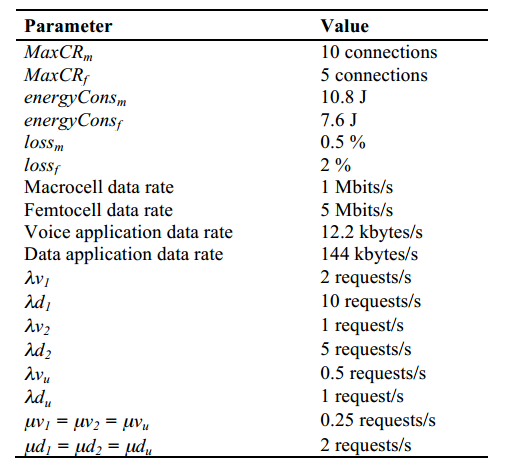
\includegraphics [width=0.45\textwidth]{./Figures/val_1}
  \end{figure} 
    \item \scriptsize Em cada cenário é analisado somente uma variável de saída.
    \item \scriptsize Durante a avaliação a variável analisada tem seu custo definido com valor 1 e as demais com valor 0.
  \end{itemize}    
\end{frame}

\begin{frame}{Descrição dos cenários}
  \begin{block}{\footnotesize Cenário 1. (SCEN1)}
    \begin{itemize}
      \item \footnotesize \alert{Objetivo:} Minimizar  o custo de consumo de energia. Método similar ao implementado pelas operadoras de comunicação atuais utilizando a rede com melhor potencia de sinal.
    \end{itemize}
  \end{block}
  
  \begin{block}{\footnotesize Cenário 2. (SCEN2)}
    \begin{itemize}
      \item \footnotesize \alert{Objetivo:} Maximizar o uso da rede baseado no melhor desempenho na taxa de transferência como critério.
    \end{itemize}
  \end{block}

  \begin{block}{\footnotesize Cenário 3. (SCEN3)}
    \begin{itemize}
      \item \footnotesize \alert{Objetivo}: Maximizar o uso da rede com melhor qualidade de serviço oferecida ao usuário , estabilidade de sinal.
    \end{itemize}
  \end{block}
\end{frame}

\begin{frame}{Descrição dos cenários}
  \begin{block}{Tabela exibindo os parâmetros dos três cenários:}
    \begin{itemize}
      \item \scriptsize Custo de energia.
      \item \scriptsize Custo da perda de voz.
      \item \scriptsize Custo da perda de dados.
      \item \scriptsize Custo taxa de transf. voz.
      \item \scriptsize Custo taxa de transf. dados.
    \end{itemize}    
  \end{block}
   
    \begin{figure}
      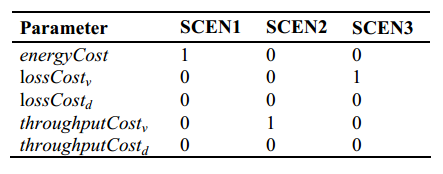
\includegraphics [width=0.65\textwidth]{./Figures/val_2}
    \end{figure}
\end{frame}

\begin{frame}{Resultado da avaliação}
  \begin{itemize}
    \item Resultados obtidos para os cenários avaliados, analisando as seguintes variáveis conforme a tabela:
  \end{itemize}
  \begin{figure}
    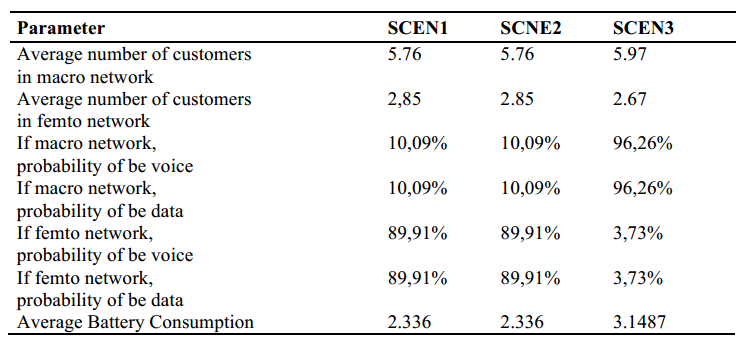
\includegraphics [width=0.75\textwidth]{./Figures/val_3}
  \end{figure}
\end{frame}

\begin{frame}
  \begin{block}{Resultado da avaliação}
    \begin{itemize}
      \item \footnotesize Nos cenários SCEN1 e SCEN2 conforme a tabela, os resultados são equivalentes, devido a rede femtocell ter os atributos preferenciais como potência do sinal e taxa de transferência.
      \newline
      \item \footnotesize Sendo \alert{89,1\%} das requisições atendidas pela rede femto e \alert{10,9\%} ser atendido pela rede macro.
      \newline
      \item \footnotesize Já em SCEN3 a rede macroCell atingiu \alert{96,26\%} das requisições devido ao baixo percentual de perda de \alert{0,5\%} enquanto da rede femto é de \alert{2\%}.
      \newline
      \item \footnotesize O custo de energia em SCEN3 sofreu alteração devido a distancia do transmissor e a rede macroCell ser a preferencial para as conexões já que é avaliado a qualidade do serviço, aumentando em \alert{25,79\%} o consumo de energia.
    \end{itemize}
  \end{block}
\end{frame}


\section{Resultados}
\frame{\tableofcontents[currentsection]}
\begin{frame}
  \begin{block}{Custos utilizados no experimento}
    \begin{figure}
      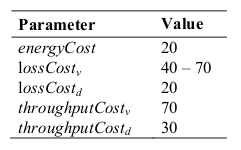
\includegraphics[scale=0.47]{./Figures/costsTable}
    \end{figure}
  \end{block}
  \begin{block}{Função custo}
    \begin{figure}
      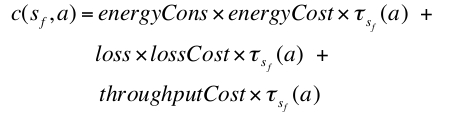
\includegraphics[scale=0.37]{./Figures/form4}
    \end{figure}
  \end{block}
  Custos não possuem dimensões. São utilizados para indicar o peso de cada
  parâmetro na função
\end{frame}

\begin{frame}{Análise da política ótima}
  \textit{Voice loss cost}
  \begin{block}{$ \text{lossCost}_v = 40$}
    \begin{itemize}
      \item Todas as requisições são atendidas pela \textit{femtocell}, até o
      seu limite de usuários
    \end{itemize}
  \end{block}
  \begin{block}{$40 < \text{lossCost}_v < 70$}
    \begin{itemize}
      \item Escolha da célula influenciada pelo grau de congestionamento da
      \textit{femtocell}
      \begin{itemize}
        \item $CR_f$ baixo: \textit{femtocell}
        \item $CR_f$ alto: \textit{macrocell}
      \end{itemize}
    \end{itemize}
  \end{block}
  \begin{block}{$\text{lossCost}_v = 70$}
    \begin{itemize}
      \item Voz e dados devem utilizar a \textit{macrocell}, a menos que esta
      esteja congestionada
    \end{itemize}
  \end{block}
\end{frame}

%\begin{frame}
%  Aumento do custo de perda, diminui importância do custo de consumo de energia
%  \begin{figure}[h]
%  	\begin{center}
%      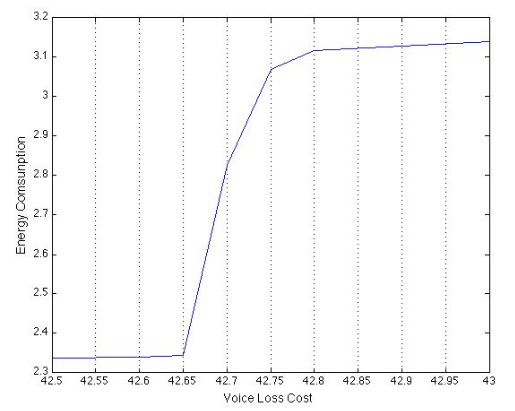
\includegraphics [scale=0.4]{./Figures/powerVSloss}
%      \caption {Consumo médio de bateria X custo de perdas de voz
%      \cite{green-markov}.}
%  		%\label{fig:arq-imuno}
%  	\end{center}
%  \end{figure}
%\end{frame}

\begin{frame}
  Aumento do custo de perda, diminui importância do custo de consumo de energia
	\begin{figure}[!htb]
		\centering
		\subfloat[Consumo vs $\textit{lossCost}_v$]{
			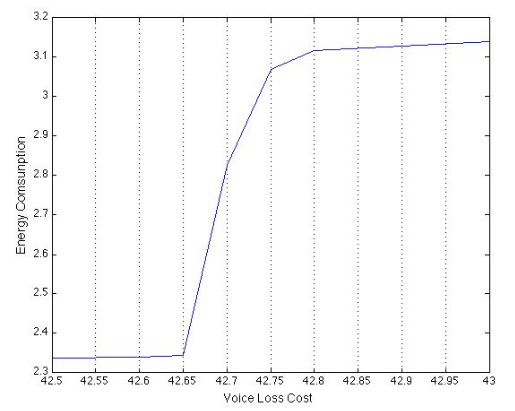
\includegraphics[height=3.9cm]{./Figures/powerVSloss}
%      \caption {Consumo médio de bateria X custo de perdas de voz
%      \cite{green-markov}.}
			\label{figdroopy}}
		\quad %espaco separador
		\subfloat[Comportamento probabilístico $\textit{lossCost}_v$]{
			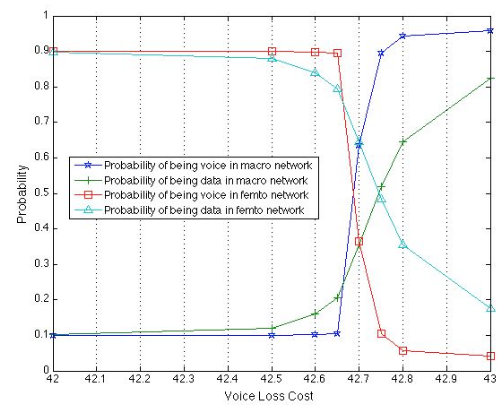
\includegraphics[height=3.9cm]{./Figures/lossProbabilities}
%      \caption {Comportamento de probabilidades \cite{green-markov}.}
			\label{figsnoop}}
		%\caption{Subfiguras}
		%\label{fig01}
	\end{figure}
  Quando o $\text{lossCost}_v = 42.7$, fluxo dividido (SCEN4).
\end{frame}

\begin{frame}
  \begin{block}{Recapitulando}
    \begin{itemize}
      \item SCEN1: Prioriza eficiência energética (intensidade de sinal)
      \item SCEN3: Prioriza QoS (vazão)
      \item SCEN4: Fluxo dividido
    \end{itemize}
  \end{block}
\end{frame}

\begin{frame}{Resultados}
  \begin{figure}[h]
  	\begin{center}
      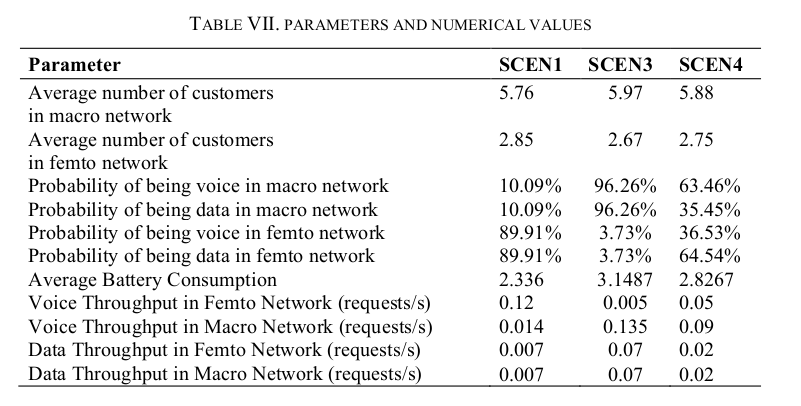
\includegraphics [scale=0.34]{./Figures/results}
     % \caption {Estimativa de dispositivos conectados à Internet.}
  		%\label{fig:arq-imuno}
  	\end{center}
  \end{figure}
  \begin{block}{Eficiência energética}
    \begin{itemize}
      \item SCEN4 aumenta $\approx 21\%$ em relação a SCEN1
      \item SCEN4 reduz em $\approx 10.22\%$ em relação a SCEN3
    \end{itemize}
  \end{block}
\end{frame}

\begin{frame}{Resultados}
  \begin{figure}[h]
  	\begin{center}
      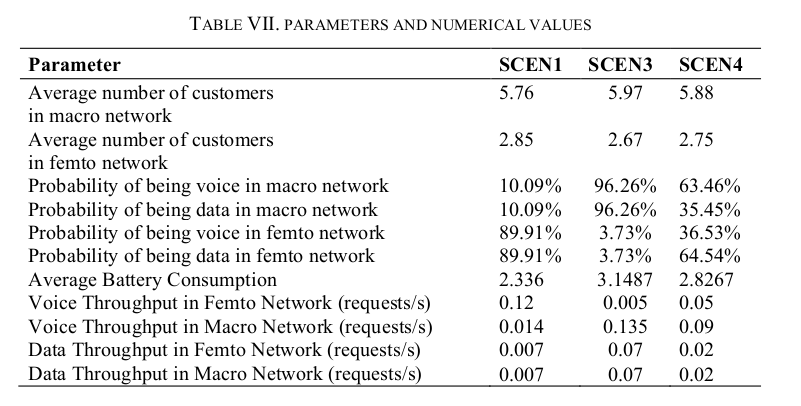
\includegraphics [scale=0.34]{./Figures/results}
     % \caption {Estimativa de dispositivos conectados à Internet.}
  		%\label{fig:arq-imuno}
  	\end{center}
  \end{figure}
  \begin{block}{Distribuição de carga - SCEN4 - Chamdas de Voz}
    \begin{itemize}
      \item \textit{macrocell}: $\approx 64\%$ ($loss = 0.5\%$, aceitável até
      $1\%$)
      \item \textit{femtocell}: $\approx 35\%$ ($loss = 2\%$)
    \end{itemize}
  \end{block}
\end{frame}

\begin{frame}{Resultados}
  \begin{figure}[h]
  	\begin{center}
      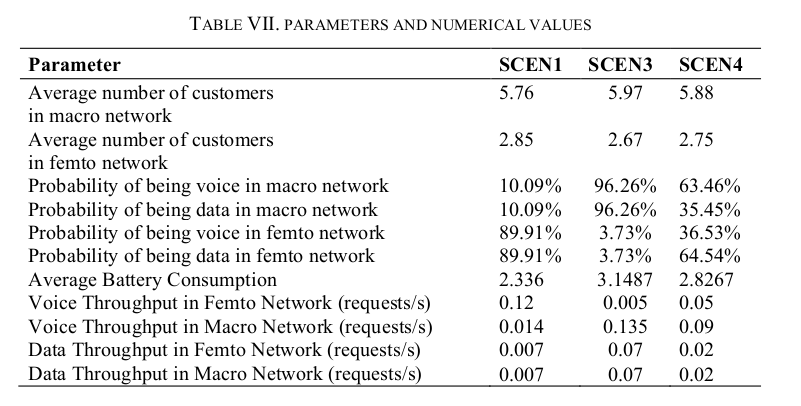
\includegraphics [scale=0.34]{./Figures/results}
     % \caption {Estimativa de dispositivos conectados à Internet.}
  		%\label{fig:arq-imuno}
  	\end{center}
  \end{figure}
  \begin{block}{Distribuição de carga - SCEN4 - Dados}
    \begin{itemize}
      \item Distribuição oposta
      \item Esperado pois a \textit{famtocell} tem melhor vazão
    \end{itemize}
  \end{block}
\end{frame}

\begin{frame}{Resultados}
  \begin{block}{}
    \begin{itemize}
      \item A política ótima proposta mantém alto nível de qualidade de
      serviço, enquanto minimiza o consumo de energia
      \item Balanceamento dos conceitos de \textit{Green Network} e
      \textit{Quality of Service}
    \end{itemize}
  \end{block}
\end{frame}

%\begin{frame}
%  \begin{block}{}
%    \begin{itemize}
%      \item
%    \end{itemize}
%  \end{block}
%\end{frame}

%\begin{frame}
%  \begin{block}{}
%  \end{block}
%\end{frame}

%\begin{frame}
%  \begin{figure}[h]
%  	\begin{center}
%      \includegraphics [scale=0.3]{./Figures/Device-Estimates}
%     % \caption {Estimativa de dispositivos conectados à Internet.}
%  		%\label{fig:arq-imuno}
%  	\end{center}
%  \end{figure}
%\end{frame}

%\begin{frame}{Redes de Acesso}
%	\begin{figure}[!htb]
%		\centering
%		\subfloat[DSL]{
%			\includegraphics[height=3.5cm]{./Figures/DSLaccess}
%			\label{figdroopy}}
%		\quad %espaco separador
%		\subfloat[Cable]{
%			\includegraphics[height=3.5cm]{./Figures/CableAccess}
%			\label{figsnoop}}
%		%\caption{Subfiguras}
%		%\label{fig01}
%	\end{figure}
%\end{frame}

%\begin{frame}[fragile]
%\scriptsize
%\begin{verbatim}
%\end{verbatim}
%\end{frame}


\section{Conclusões}
\frame{\tableofcontents[currentsection]}
\begin{frame}{Conclusões}
  \begin{block}{}
    \begin{itemize}
      \item \textit{Femtocells} permitem um \alert{aumento de cobertura}
      celular, além da \alert{diminuição} da carga em \textit{Macrocells}, a um
      \alert{baixo custo}, contudo:
      \begin{itemize}
        \item alocação ótima de clientes ainda é um problema em aberto
        \item ainda mais complexo quando consideradas questões de eficiência
        energética
      \end{itemize}
    \end{itemize}
  \end{block}
  \pause
  \begin{block}{}
    \begin{itemize}
      \item Através de alocação ótima, o artigo busca oferecer os
      \alert{melhores níveis de serviço}, ao mesmo tempo que visa
      \alert{maximizar a vida útil da bateria}
      \begin{itemize}
        \item considera características dos tipos de serviço (voz/dados)
      \end{itemize}
    \end{itemize}
  \end{block}
\end{frame}

\begin{frame}{Resultados}
  \begin{block}{Obervações}
    \begin{itemize}
      \item Conexões de \alert{voz} devem ser direcionadas para
      \alert{\textit{macrocells}}
      \begin{itemize}
        \item Maior capacidade de clientes
        \item Maior cobertura
        \item Menores indices de perdas
      \end{itemize}
      \item Conxões de \alert{dados} devem ser direcionadas para
      \alert{\textit{femtocells}}
      \begin{itemize}
        \item Maior largura de banda
        \item Apesar das perdas, atende requisitos de QoS para dados (TCP/IP)
      \end{itemize}
    \end{itemize}
  \end{block}
\end{frame}

\begin{frame}{Resultados}
  \begin{block}{Contribuições}
    \begin{enumerate}
      \item Proposta de um modelo de alocação ótima
      \item Consideração de aspectos de diferentes camadas (nível de sinal,
      eficiência energética)
      \item \textit{Green Markov Library}
    \end{enumerate}
  \end{block}
\end{frame}

%\begin{frame}
%  \begin{block}{}
%    \begin{itemize}
%      \item
%    \end{itemize}
%  \end{block}
%\end{frame}

%\begin{frame}
%  \begin{block}{}
%  \end{block}
%\end{frame}

%\begin{frame}
%  \begin{figure}[h]
%  	\begin{center}
%      \includegraphics [scale=0.3]{./Figures/Device-Estimates}
%     % \caption {Estimativa de dispositivos conectados à Internet.}
%  		%\label{fig:arq-imuno}
%  	\end{center}
%  \end{figure}
%\end{frame}

%\begin{frame}{Redes de Acesso}
%	\begin{figure}[!htb]
%		\centering
%		\subfloat[DSL]{
%			\includegraphics[height=3.5cm]{./Figures/DSLaccess}
%			\label{figdroopy}}
%		\quad %espaco separador
%		\subfloat[Cable]{
%			\includegraphics[height=3.5cm]{./Figures/CableAccess}
%			\label{figsnoop}}
%		%\caption{Subfiguras}
%		%\label{fig01}
%	\end{figure}
%\end{frame}

%\begin{frame}[fragile]
%\scriptsize
%\begin{verbatim}
%\end{verbatim}
%\end{frame}


%\section{Referências}
%\frame{\tableofcontents[currentsection]}

\begin{frame}[allowframebreaks]{Referências}
% \bibliography{../referencias}

\begin{thebibliography}{10}
		\bibitem{green-markov}[1]
			Green-Markov models-new optimization strategies: a case study
      for user allocation in co-channel macro/femto networks
      \newblock Cardoso, Diego L and Santana, Adamo L de and Silva, Marcelino S da and
      Franc{\^e}s, Carlos RL and Costa, Jo{\~a}o CWA and Carvalho, Solon V de
      and Vijaykumar
			\newblock Journal of Microwaves, Optoelectronics and Electromagnetic
      Applications, 2012
		%\bibitem{class}[2]
		%	Author name
		%	\newblock Title.
		%	\newblock Conference, 2018.
\end{thebibliography}
\end{frame}

\begin{frame}{Dúvidas?}
  \begin{figure}[h]
  	\begin{center}
      \includegraphics [scale=0.4]{./Figures/duvida}
      %\caption {Modelagem Geral do Sistema Imuno.}
  		%\label{fig:arq-imuno}
  	\end{center}
  \end{figure}
\end{frame}

%\begin{frame}
%	\begin{block}{}
%		\begin{center}
%			\textbf{Obrigado pela aten\c{c}\~{a}o!}
%		\end{center}
%	\end{block}
%	\begin{itemize}
%  		\item andresp@lasca.ic.unicamp.br
%  	\end{itemize}
%	\vspace{2cm}
%\end{frame}


\end{document}
